%%%%%%%%%%%%%%%%%%%%%
% Version 1 17/10/25


\documentclass[12pt,a4paper,openany,twoside]{book}
\usepackage[top=1in, bottom=1in, left=0.8in, right=0.8in]{geometry} % 0.8 inch margins

% Language and date format
\usepackage[UKenglish]{babel} 
\usepackage[UKenglish]{isodate}
\cleanlookdateon 

% Fonts
\usepackage[T1]{fontenc} %DO NOT CHANGE
\usepackage{lmodern} % better Latin Modern fonts %DO NOT CHANGE
\usepackage{microtype} % improves justification and kerning 

% Graphics and captions
\usepackage{graphicx} 
\usepackage[dvipsnames]{xcolor} % Gives you colours! 
\usepackage[margin=15pt,font=footnotesize,labelfont=bf,format=hang]{caption} 
\usepackage{subcaption} 
\usepackage{pgfplots} % you can import graphs as PGF files 
\pgfplotsset{compat=1.18} 
\usepackage{float}

% Maths
\usepackage{amsmath,amssymb,mathtools} 
\usepackage{bm} % Making letters bold 
\usepackage{isomath} % Modern standards

% Labelled matrices
\usepackage{nicematrix}

% Chemical Formulae
\usepackage{mhchem}

% Theorems, definitions, etc.
\usepackage{amsthm} 
\newtheorem{theorem}{Theorem}[chapter] % Number theorem per chapter
\newtheorem{lemma}[theorem]{Lemma} % Number lemmas like theorems
\newtheorem{definition}{Definition}[chapter] % Number definitions per chapter

% Lists, tables, units
\usepackage{enumitem} % Allows for formatting of lists 
\setlist{topsep=0pt} 
\usepackage{booktabs} % Prettier tables 
\usepackage{siunitx} % Typeset measurements correctly 

% Referencing
\usepackage{natbib}

\bibliographystyle{abbrvnat} % possible citation style
%\bibliographystyle{plain} % possible citation style
%\setcitestyle{authoryear,open={(},close={)}} % Many options available. Can be changed after discussing with your supervisor.
\usepackage[pdfencoding=auto,pdftitle={Dissertation},pdflang={en-GB}]{hyperref} % Make links work
\hypersetup{
	colorlinks = true,
	linkcolor = black,
	citecolor = black
}
\usepackage{cleveref} % Easy internal referencing 

% Formatting
\usepackage[raggedright]{titlesec} %DO NOT CHANGE
\usepackage{fancyhdr} %DO NOT CHANGE

%% Subfiles so you can write separate chapter files [You can enable this if you're using subfiles]
%\usepackage{subfiles}
%\newcommand{\subfilebibliography}{%
%	\ifSubfilesClassLoaded{%
%		\bibliography{references.bib}
%	}{}
%} % Makes the bibliography work for every chapter file

% Headers and footers. 
\pagestyle{fancy} %DO NOT CHANGE
\renewcommand{\headrulewidth}{0pt} %DO NOT CHANGE
\renewcommand\sectionmark[1]{\markright{\thesection\; #1}} %DO NOT CHANGE
\fancyhead[RO]{\small\it\lowercase\nouppercase\selectfont\rightmark} %DO NOT CHANGE
\fancyhead[LO]{}%DO NOT CHANGE
\fancyhead[LE]{\small\it\lowercase\nouppercase\selectfont\rightmark} %DO NOT CHANGE
\fancyhead[RE]{} %DO NOT CHANGE
\setlength{\headheight}{15pt} %DO NOT CHANGE
\fancypagestyle{blank}{\fancyhf{}\fancyfoot[C]{}\renewcommand{\headrulewidth}{0pt}} %DO NOT CHANGE

% Standard spacing
\setlength{\parindent}{0ex} %DO NOT CHANGE
\setlength{\parskip}{1ex} %DO NOT CHANGE
\let\cleardoublepage\clearpage %DO NOT CHANGE


% Chapter title
\titleformat{\chapter}[display] %DO NOT CHANGE
{\Huge\bfseries}   % font size and style %DO NOT CHANGE
{\chaptername\ \thechapter} % label %DO NOT CHANGE
{20pt}             % spacing between label and title %DO NOT CHANGE
{\Huge}            % title formatting %DO NOT CHANGE

\titlespacing*{\chapter} %DO NOT CHANGE
{0pt}    % left margin %DO NOT CHANGE
{0pt}   % space before chapter title %DO NOT CHANGE
{20pt}   % space after chapter title %DO NOT CHANGE

% Section title %DO NOT CHANGE
\titleformat{\section} %DO NOT CHANGE
{\large\bfseries}  % font size and style %DO NOT CHANGE
{\thesection}      % label %DO NOT CHANGE
{1em}              % spacing between label and title %DO NOT CHANGE
{} %DO NOT CHANGE

\titlespacing*{\section} %DO NOT CHANGE
{0pt}    % left margin %DO NOT CHANGE
{10pt}   % space before section title %DO NOT CHANGE
{10pt}   % space after section title %DO NOT CHANGE

% Subsection title %DO NOT CHANGE
\titleformat{\subsection} %DO NOT CHANGE
{\normalsize\bfseries}  % font size and style %DO NOT CHANGE
{\thesubsection}      % label %DO NOT CHANGE
{1em}              % spacing between label and title %DO NOT CHANGE
{}

\titlespacing*{\subsection} %DO NOT CHANGE
{0pt}    % left margin %DO NOT CHANGE
{10pt}   % space before subsection title %DO NOT CHANGE
{0pt}   % space after subsection title %DO NOT CHANGE


%From here you can find useful commands to save time and make things look nice. You can use them, change them, or add to them at will

% Vectors, matrices etc.
\renewcommand{\v}[1]{\mathbf{#1}}      % Generic vector
\newcommand{\uv}[1]{\widehat{\mathbfit{#1}}}      % Generic unit vector
\renewcommand{\t}[1]{\mathsfbfit{#1}}	 % Generic tensor
\newcommand{\m}[1]{\bm{\mathsf{#1}}}	 % Generic matrix
\newcommand{\tu}[1]{\bm{\mathsf{#1}}}	 % Upright tensor (for zero tensor)

%Vector operators
\renewcommand{\d}{{\mathrm d}}
\def \p {\partial}
\newcommand{\vnabla}{\bm{\nabla}}
\newcommand{\Lap}{{\Delta}} %Pure Laplacian
\newcommand{\aLap}{\nabla^2} %Applied Laplacian
%Hats, tildes and bars that fit
\renewcommand{\hat}{\widehat}
\renewcommand{\tilde}{\widetilde}
\renewcommand{\bar}{\overline}

% Differentiating 
\newcommand{\fd}[2]{\mathchoice{\frac{\d #1}{\d #2}}{\d #1/\d #2}{\d #1/\d #2}{\d #1/\d #2}}
\newcommand{\fdd}[2]{\mathchoice{\frac{\d^2 #1}{\d #2^2}}{\d^2 #1/\d #2^2}{\d^2 #1/\d #2^2}{\d^2 #1/\d #2^2}}
\newcommand{\fddd}[2]{\mathchoice{\frac{\d^3 #1}{\d #2^3}}{\d^3 #1/\d #2^3}{\d^3 #1/\d #2^3}{\d^3 #1/\d #2^3}}
\newcommand{\fdddd}[2]{\mathchoice{\frac{\d^4 #1}{\d #2^4}}{\d^4 #1/\d #2^4}{\d^4 #1/\d #2^4}{\d^4 #1/\d #2^4}}
\newcommand{\fdn}[3]{\mathchoice{\frac{\d^{#1} #2}{\d #3^{#1}}}{\d^{#1} #2/\d #3^{#1}}{\d^{#1} #2/\d #3^{#1}}{\d^{#1} #2/\d #3^{#1}}}
\newcommand{\pd}[2]{\mathchoice{\frac{\p #1}{\p #2}}{\p #1/\p #2}{\p #1/\p #2}{\p #1/\p #2}}
\newcommand{\pdd}[2]{\mathchoice{\frac{\p^2 #1}{\p #2^2}}{\p^2 #1/\p #2^2}{\p^2 #1/\p #2^2}{\p^2 #1/\p #2^2}}
\newcommand{\pddmixed}[3]{\mathchoice{\frac{\p^2 #1}{\p #2 \p #3}}{\p^2 #1 /\p #2 \p #3}{\p^2 #1 /\p #2 \p #3}{\p^2 #1 /\p #2 \p #3}}
\newcommand{\pddd}[2]{\frac{\p^3 #1}{\p #2^3}}
\newcommand{\pdn}[3]{\mathchoice{\frac{\p^{#1} #2}{\p #3^{#1}}}{\p^{#1} #2/\p #3^{#1}}{\p^{#1} #2/\p #3^{#1}}{\p^{#1} #2/\p #3^{#1}}}

% Misc
\DeclareMathSymbol{\Delta}{\mathalpha}{operators}{1} % Keeps Delta upright
\DeclareMathSymbol{\Gamma}{\mathalpha}{operators}{0} % Keeps Gamma upright
\newcommand{\ep}{\varepsilon} % A more normal epsilon

% Upright e and i for exponential and imaginary number
\newcommand{\e}{\mathrm{e}}
\renewcommand{\i}{\mathrm{i}}

	
\begin{document} %DO NOT REMOVE the title page. Just edit it.
\frontmatter
	% Pretty title page
	\thispagestyle{empty}
	\begin{titlepage}
		\begin{center}
			
\includegraphics[scale=0.8]{figs/durham-logo.pdf}
			\vspace{45mm}
			
			\Huge \textbf{All your nodes are belong to us: An exploration of percolation-like disease modelling.}
			
			\vspace{15mm}
			\large
			\begin{align*}
				\textit{by} &\quad \text{Matthew Evans} \\[4mm]
				\textit{Supervisor} &\quad \text{Dr Andrew Krause}
			\end{align*}
			\vspace{35mm}
			
			A dissertation submitted for the degree of \\
			\emph{MMath Mathematics}
			\vspace{5mm}
			
			\today
		\end{center}
	\end{titlepage}
	\normalsize
	
	% ----- PLAGIARISM DECLARATION ----- 
        % DO NOT REMOVE. WRITE YOUR NAME IN THE APPROPRIATE PLACE TO ACKNOWLEDGE THAT YOU HAVE READ, HAVE UNDERSTOOD, AND CONFIRM THAT YOU ADHERE TO THE STATEMENT.
	\begin{center}
		\large\textbf{Plagiarism declaration}
	\end{center}
	\begin{quote}
		This piece of work is a result of my own work and I have complied with the Department’s guidance on multiple submission and on the use of AI tools. Material from the work of others not involved in the project has been acknowledged, quotations and paraphrases suitably indicated, and all uses of AI tools have been declared.
	\end{quote}
	\vfill
	I, \underline{Matthew Evans} confirm that I have read, understood, and have adhered to the plagiarism declaration above.
	
	\newpage
	
		% ----- Declaration of use of AI tools in the writing process. ----- DO NOT REMOVE. Fill as needed 
	\begin{center}
		\large\textbf{Declaration of use of AI tools in the writing process}
	\end{center}
	\begin{center}
                No AI tools were used in this project, for any purpose.
	\end{center}
	
	
	\newpage
	
	% ----- ABSTRACT ----- % You may remove if you want or modify upon agreement with your supervisor
	\begin{center}
		\large\textbf{Abstract}
	\end{center}
	\begin{quote}
                TODO: write one of these
	\end{quote}
	
	\newpage
	
	% ----- ACKNOWLEDGEMENTS ----- % You may remove if you want or modify upon agreement with your supervisor

	% ----- LIST OF FIGURES ----- % You may remove if you want or modify upon agreement with your supervisor
	
	\listoffigures
	\markboth{}{} 
	%	The name of the figure that appears in the list is taken from the short description of the caption, i.e.
	% \caption[short caption - appears in the list of figures]{long caption - appears under the figure}
	% if no short description appears, i.e. if you use \caption{something} then 'something' will appear in the list of figures (and might be a very long sentence!).
	
	\newpage
	
	% ----- LIST OF TABLES----- % You may remove if you want or modify upon agreement with your supervisor
	
	\listoftables
	\markboth{}{} 
	% You will need to use the Table environment (not Tabular) and to use \caption in order for the table to appear in the above list (you can wrap the tabular environment within a table environemnt, see an example below). Much like with the list of figures, the short description of the caption is the one that is taken for the list of tables. 
	
	\newpage
	
	% ----- LIST OF NOTATION----- % You may remove if you want or modify upon agreement with your supervisor
	
	\chapter*{Notation}

	
	\begin{tabular}{p{4cm} l  }
	\end{tabular}
	
	
	% Pretty table of contents - DO NOT CHANGE OR REMOVE
	\setlength{\parskip}{0.2ex}
	\setcounter{tocdepth}{1}
	\renewcommand{\baselinestretch}{0.95}\normalsize
	\tableofcontents
	\renewcommand{\baselinestretch}{1}\normalsize
	\markboth{}{} 
	\setlength{\parskip}{1ex}
	

\mainmatter

\chapter{Introduction}

Throughout human history, disease has been one of the greatest societal challenges. From the black death, to COVID-19, widespread infection has disrupted society, caused economic recessions, and caused suffering to millions of people \citep{prabhuHistorysSevenDeadliest}. It is therefore no surprise that Epidemiology has a rich and vaired history, as we have tried to understand diseases from their chemical functions, to their effect on the human body, to how they spread through a population. It is this last problem which this report is concerned with.

Disease modelling has the potential to impact governmental policy with regards to pandemic preparedness and responses, as well as outbreak containment and response \citep{gov.ukEpidemiologicalModellingFrequently}. It is clearly of great importance to develop accurate and realistic models for disease spread, and for these to be flexible enough to be effective in their use \citep{lancetHowModellingCan2024}. It is also important to make these models easy to interpret and communicate to the general public. The effectiveness of this was evident during the COVID-19 pandemic, as a great number of people were encouraged to ``flatten the curve'' - a direct reference to the underlying models used to predict the effect of the pandemic \citep{ecdcVideoCOVID19Flatten2020}.

Now the effects of the COVID-19 pandemic are waning, and so it is important to build upon the huge amount of work that was done at the time, to develop more accurate and useful models for other diseases with different attributes, such as passive immunity from birth. These models can help to shape public policy surrounding not just pandemics and outbreaks, but also vaccination programmes, and other forms of aid globally.

\chapter{The SI Model}

\section{Naïve SSA}

A Naïve approach was first implemented in order to evaluate whether the spreading algorithm would behave as expected. This was achieved by defining a set of state vectors, which for the most basic SI model we denote $\v{S}(t)$ and $\v{I}(t)$. The state vectors behave such that $S_i = 1$ if node $i$ is in the Susceptible compartment, and $I_i = 1$ if node $i$ is in the Infectious compartment. Further, we define $S_i = 0$ or $I_i = 0$ for node $i$ not in the Susceptible or Infectious compartments, respectively. We therefore have as a result that $S_i + I_i = 1 \quad \forall \, i$. The time $t$ is also logged. On each step, the value of $\v{I}(t)$ is stored in a temporary vector, for comparison later. The infection is then spread according to the formulae

\begin{align}
	\v{I}(t + \Delta t) &= \Theta(\v{I}(t) + \m{A} \cdot \v{I}(t) * \v{S}(t)), \\
	\v{S}(t + \Delta t) &= \Theta(\v{S}(t) - \v{I}(t + \Delta t)),
\end{align}

where $*$ denotes component-wise multiplication between vectors and $\Theta$ is the discrete Heaviside function applied to each component where

\begin{equation*}
	\Theta =
	\begin{cases*}
		0 & \text{if} n $\leq$ 0, \\
		1 & \text{if} n > 0.
	\end{cases*}
\end{equation*}

This is the very simple and naïve process whereby the infection simply spreads from all infected nodes to any susceptible neighbours, in a discrete time step $\Delta t$. The simulation ends when $\v{I}(t + \Delta t) = \v{I}(t)$. This was enough to be able to demonstrate the effectiveness of the code and confirm that the graph generation and spreading worked.

\section{Gillespie SI}

\section{Comparison of networked SI models to well-mixed SI}

Having implemented this algorithm, we can now compare the networked implementation of the SI model to a standard Gillespie SSA simulation of a well-mixed SI model. Notably, this should be equivalent to the network Gillespie on the $K_N$ graph, where $N$ is the total population. To ensure relatively easy comparison, the population size was set at 10000, or a $100 \times 100$ lattice. Each algorithm was iterated $20$ times, tracking the infected populations. All of the trajectories thus generated were then plotted. We set the parameters at $p \in \{0.3, 0.5, 0.7 \}$ as the chance of an edge existing in the graph, and $k_I = 0.5$ as the infection rate. For the well-mixed algorithm, we chose $k_I = 0.00002$. This was to ensure the plots were more easily comparable, as the low average degree of a percolation-type graph greatly reduces the effective infection rate relative to the well-mixed version.

As one would expect, the well-mixed SI model shows logistic-curve-like behaviour, and all individuals eventually become infected. However, for the graph-based model, we see qualitatively different behaviour, with very different results for different values of $p$. For the subcritical graph with $p = 0.3$, we see approximately linear behaviour, and a considerably smaller fraction of the total population is infected. This is due to the low connectivity of the graph resulting in the infection being confined to small connected components of the graph. For the critical graph, with $p = 0.5$, we again see approximately linear behaviour, with some trailing off near the end of most infectionsv. We also observe a far greater proportion of the overall population becoming infected, corresponding to a large connected component of the graph existing. In some cases, the component containing the initial infection is small, and so a far smaller proportion of the population are infected. Finally, in the supercritical case where $p = 0.7$, we see again almost the entire population are eventually infected. There is also some trace of logistic-like properties, with the infection rate being highest when approximately half of the population is infected. However, the slower initial and final rates are less pronounced than in the well-mixed case, and the lines are more easily approximated with a linear best fit than the traces resulting from the well-mixed model. In this condition, the eventual spread. looks similar to the case on a complete lattice (where every edge exists).

This difference in behaviour is partially a result of the approximately circular wavefront of the infection. Clearly the rate of infection is proportional to the length of the perimeter, which is proportional to the square root of the number of infected individuals, where in the mixed model the infection rate is proportional to the square of the number of infected (in the central region). This results in much slower growth of the infected population relative to the well-mixed model. The other factor impacting the qualitative behaviour of the different simulations is the breaks in the graph where sub populations are isolated from one another, and so the spread cannot propagate as rapidly or as far through the total population.

\begin{figure}
	\centering
	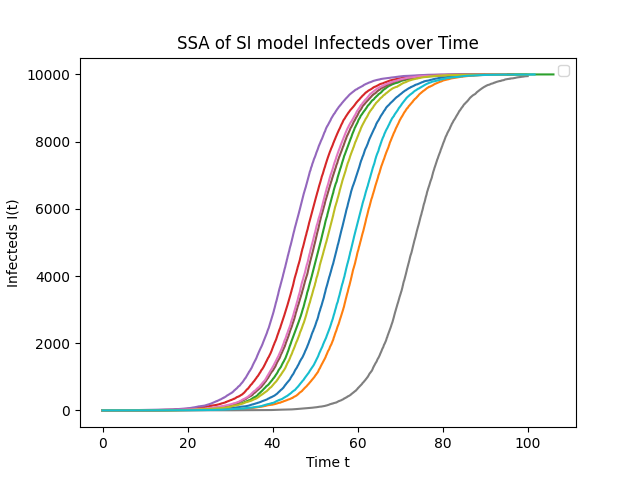
\includegraphics[width=0.7\textwidth]{figs/mixSI.png}
	\caption{Well-mixed simulation}
	\label{fig:mixSI}
\end{figure}

\chapter{Exploring other models}

We wanted to see how the criticality effects of different $p$ values on the percolation-type graphs were affected differently by different models, and so the Gillespie SSA was implemented for a variety of different models, utilising a similar process to the SI model to explore the evolution of the epidemic.

\section{The SIS Model}

\subsection{The Model}

The next most simple model is the SIS model, which is an accurate portrayal of various STIs, wherein an individual can be infected by another infected individual, and can later become uninfected, but they do not ever become immune to the disease. This is represented by the system

\begin{equation}
	\ce{S + I ->[k_I] 2I} \qquad \ce{I ->[k_U] S}.
\end{equation}

Here, $k_I$ is still the infection rate, and $k_U$ is the rate of recovery without immunity. Once again, we implemented a well-mixed Gillespie SSA as well as the graph-based models. 

\begin{figure}
	\centering
	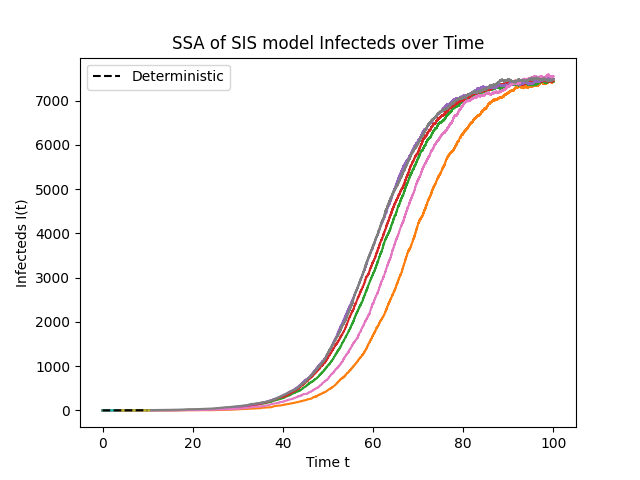
\includegraphics[width=0.7\textwidth]{figs/mixSIS.png}
	\caption{Well-mixed simulation}
	\label{fig:mixSIS}
\end{figure}

\bibliography{mybib.bib}

\end{document}